\documentclass[12pt, titlepage]{article}

\usepackage{fullpage}
\usepackage[round]{natbib}
\usepackage{multirow}
\usepackage{booktabs}
\usepackage{tabularx}
\usepackage{graphicx}
\usepackage{float}
\usepackage{hyperref}
\hypersetup{
    colorlinks,
    citecolor=blue,
    filecolor=black,
    linkcolor=red,
    urlcolor=blue
}

\input{../../Comments.text}
\input{../../Common.text}


\newcounter{acnum}
\newcommand{\actheacnum}{AC\theacnum}
\newcommand{\acref}[1]{AC\ref{#1}}

\newcounter{ucnum}
\newcommand{\uctheucnum}{UC\theucnum}
\newcommand{\uref}[1]{UC\ref{#1}}

\newcounter{mnum}
\newcommand{\mthemnum}{M\themnum}
\newcommand{\mref}[1]{M\ref{#1}}

\begin{document}

\title{Module Guide for \progname{}} 
\author{\authname}
\date{\today}

\maketitle

\pagenumbering{roman}

\section{Revision History}

\begin{tabularx}{\textwidth}{p{3cm}p{2cm}X}
\toprule {\bf Date} & {\bf Version} & {\bf Notes}\\
\midrule
Apr 22, 2026 & 1.2 & Addressed peer review feedback on TRF computation backend ownership\\
Mar 25, 2026 & 1.1 & Post-presentation refinements based on professor's feedback; remove software decision module; align with feedback\\
March 5, 2026 & 1.0 & Initial Draft\\
\bottomrule
\end{tabularx}

\newpage

\section{Reference Material}

This section records information for easy reference. 

\subsection{Abbreviations and Acronyms}

\renewcommand{\arraystretch}{1.2}
\begin{tabular}{l l}
  \toprule
  \textbf{symbol} & \textbf{description}\\
  \midrule
  A & Assumption\\
  DD & Data Definition\\
  GD & General Definition\\
  GS & Goal Statement\\
  IM & Instance Model\\
  LC & Likely Change\\
  PS & Physical System Description\\
  R & Requirement\\
  SRS & Software Requirements Specification\\
  \progname{} & software system that loads MEG/EEG experimental data, configures NCRF/TRF estimators, and computes stimulus–response TRFs within a flexible analysis pipeline\\
  TM & Theoretical Model\\
  \bottomrule
\end{tabular}\\

\newpage

\tableofcontents

\listoftables

\listoffigures

\newpage

\pagenumbering{arabic}

\section{Introduction}

Decomposing a system into modules is a commonly accepted approach to developing
software.  A module is a work assignment for a programmer or programming
team~\citep{ParnasEtAl1984}.  We advocate a decomposition
based on the principle of information hiding~\citep{Parnas1972a}.  This
principle supports design for change, because the ``secrets'' that each module
hides represent likely future changes.  Design for change is valuable in SC,
where modifications are frequent, especially during initial development as the
solution space is explored.  

Our design follows the rules laid out by \citet{ParnasEtAl1984}, as follows:
\begin{itemize}
\item System details that are likely to change independently should be the
  secrets of separate modules.
\item Each data structure is implemented in only one module.
\item Any other program that requires information stored in a module's data
  structures must obtain it by calling access programs belonging to that module.
\end{itemize}

After completing the first stage of the design, the Software Requirements
Specification (SRS), the Module Guide (MG) is developed~\citep{ParnasEtAl1984}. The MG
specifies the modular structure of the system and is intended to allow both
designers and maintainers to easily identify the parts of the software.  The
potential readers of this document are as follows:

\begin{itemize}
\item New project members: This document can be a guide for a new project member
  to easily understand the overall structure and quickly find the
  relevant modules they are searching for.
\item Maintainers: The hierarchical structure of the module guide improves the
  maintainers' understanding when they need to make changes to the system. It is
  important for a maintainer to update the relevant sections of the document
  after changes have been made.
\item Designers: Once the module guide has been written, it can be used to
  check for consistency, feasibility, and flexibility. Designers can verify the
  system in various ways, such as consistency among modules, feasibility of the
  decomposition, and flexibility of the design.
\end{itemize}

The rest of the document is organized as follows. Section
\ref{SecChange} lists the anticipated and unlikely changes of the software
requirements. Section \ref{SecMH} summarizes the module decomposition that
was constructed according to the likely changes. Section \ref{SecConnection}
specifies the connections between the software requirements and the
modules. Section \ref{SecMD} gives a detailed description of the
modules. Section \ref{SecTM} includes two traceability matrices. One checks
the completeness of the design against the requirements provided in the SRS. The
other shows the relation between anticipated changes and the modules. Section
\ref{SecUse} describes the use relation between modules.

\section{Anticipated and Unlikely Changes} \label{SecChange}

This section lists possible changes to the system. According to the likeliness
of the change, the possible changes are classified into two
categories. Anticipated changes are listed in Section \ref{SecAchange}, and
unlikely changes are listed in Section \ref{SecUchange}.

\subsection{Anticipated Changes} \label{SecAchange}

Anticipated changes are the source of the information that is to be hidden
inside the modules. Ideally, changing one of the anticipated changes will only
require changing the one module that hides the associated decision. The approach
adapted here is called design for
change.

\begin{description}
\item[\refstepcounter{acnum} \actheacnum \label{acHardware}:] Hardware platform and OS compatibility.
\item[\refstepcounter{acnum} \actheacnum \label{acInput}:] Input data schema and storage conventions for MEG/EEG signals and predictors.
\item[\refstepcounter{acnum} \actheacnum \label{acEstimator}:] Estimator selection and parameter resolution strategy (e.g., boosting vs NCRF).
\item[\refstepcounter{acnum} \actheacnum \label{acTRF}:] TRF computation method and related estimation parameters.
\end{description}

% \wss{Anticipated changes relate to changes that would be made in requirements,
% design or implementation choices.  They are not related to changes that are made
% at run-time, like the values of parameters.}

\subsection{Unlikely Changes} \label{SecUchange}

The module design should be as general as possible. However, a general system is
more complex. Sometimes this complexity is not necessary. Fixing some design
decisions at the system architecture stage can simplify the software design. If
these decisions later need to be changed, then many parts of the design
will potentially need to be modified. Hence, it is not intended that these
decisions will be changed.

\begin{description}
\item[\refstepcounter{ucnum} \uctheucnum \label{ucIO}:] Input/Output devices
  (Input: MEG/EEG data and predictors, Output: serialized TRF results and
  diagnostic plots/reports).
\item[\refstepcounter{ucnum} \uctheucnum \label{ucIO}:] Core TRF-based stimulus-response model.

\end{description}

\section{Module Hierarchy} \label{SecMH}

This section provides an overview of the module design. Modules are summarized
in a hierarchy decomposed by secrets in Table \ref{TblMH}. The modules listed
below, which are leaves in the hierarchy tree, are the modules that will
actually be implemented.

\begin{description}
\item [\refstepcounter{mnum} \mthemnum \label{mHH}:] Data Loading Module
\item  [\refstepcounter{mnum} \mthemnum \label{mInput}:]  Data Preprocessing Module
\item [\refstepcounter{mnum} \mthemnum \label{mEstimator}:] Estimator Resolution Module
\item [\refstepcounter{mnum} \mthemnum \label{mTRF}:] TRF Computation Module
\end{description}


\begin{table}[h!]
\centering
\begin{tabular}{p{0.3\textwidth} p{0.6\textwidth}}
\toprule
\textbf{Level 1} & \textbf{Level 2}\\
\midrule

{Hardware-Hiding Module} & Data Loading Module \\
\midrule

\multirow{3}{0.3\textwidth}{Behaviour-Hiding Module} & Data Preprocessing Module\\
& Estimator Resolution Module\\
& TRF Computation Module\\
\bottomrule

\end{tabular}
\caption{Module Hierarchy}
\label{TblMH}
\end{table}

\section{Connection Between Requirements and Design} \label{SecConnection}

The design of the system is intended to satisfy the requirements developed in
the SRS. In this stage, the system is decomposed into modules. The connection
between requirements and modules is listed in Table~\ref{TblConnection}.

\begin{table}[H]
\centering
\begin{tabular}{p{0.45\textwidth} p{0.45\textwidth}}
\toprule
\textbf{Requirements (SRS)} & \textbf{Module ID}\\
\midrule
R1 (\textit{R-Inputs}) & \mref{mInput}, \mref{mHH}\\
R2 (\textit{R-Calculate}) & \mref{mEstimator}, \mref{mTRF}\\
R3 (\textit{R-Output}) & \mref{mTRF}\\
NFR1 (\textit{Accuracy}) & \mref{mEstimator}, \mref{mTRF}\\
NFR2 (\textit{Maintainability}) & \mref{mInput}, \mref{mEstimator}, \mref{mTRF}\\
NFR3 (\textit{Portability}) & \mref{mHH}\\
\bottomrule
\end{tabular}
\caption{Connection Between Requirements and Module IDs}
\label{TblConnection}
\end{table}

% \wss{The intention of this section is to document decisions that are made
%   ``between'' the requirements and the design.  To satisfy some requirements,
%   design decisions need to be made.  Rather than make these decisions implicit,
%   they are explicitly recorded here.  For instance, if a program has security
%   requirements, a specific design decision may be made to satisfy those
%   requirements with a password.}

\section{Module Decomposition} \label{SecMD}

Modules are decomposed according to the principle of ``information hiding''
proposed by \citet{ParnasEtAl1984}. The \emph{Secrets} field in a module
decomposition is a brief statement of the design decision hidden by the
module. The \emph{Services} field specifies \emph{what} the module will do
without documenting \emph{how} to do it. For each module, a suggestion for the
implementing software is given under the \emph{Implemented By} title. If the
entry is \emph{OS}, this means that the module is provided by the operating
system or by standard programming language libraries.  \emph{\progname{}} means the
module will be implemented by the \progname{} software.

Only the leaf modules in the hierarchy have to be implemented. If a dash
(\emph{--}) is shown, this means that the module is not a leaf and will not have
to be implemented.

\subsection{Hardware Hiding Modules (\mref{mHH})}

\begin{description}
\item[Secrets:]The detailed environment implementation for the hardware.
\item[Services:] Interfaces with system hardware and filesystem for data loading.
\item[Implemented By:] OS libraries
\end{description}

\subsection{Behaviour-Hiding Module}

\begin{description}
\item[Secrets:]The workflow-level behaviours that realize the functional
  requirements (data preprocessing, TRF computation, and result preparation)
  using the experiment configuration in the TRF pipeline.
\item[Services:]Coordinates execution of the NCRF/TRF workflow through
  experiment-level operations (for example, subject selection, predictor
  availability, and TRF computation) while handling estimator selection in the
  Estimator Resolution Module. This layer isolates requirement-driven behaviour
  from core numerical implementation details.
\item[Implemented By:] --
\end{description}

\subsubsection{Data Preprocessing Module (\mref{mInput})}

\begin{description}
\item[Secrets:]The accepted schema and storage conventions for predictors and
 trial metadata.
\item[Services:]Loads and preprocesses MEG/EEG signals, validates metadata. 
\item[Implemented By:] \progname{}
\item[Type of Module:] Library
\end{description}

\subsubsection{TRF Computation Module (\mref{mTRF})}

\begin{description}
\item[Secrets:] The implementation of TRF calculation with different estimation parameters.
\item[Services:] Compute TRF model outputs given preprocessed MEG/EEG data,
  predictor signals, and estimator parameters. Returns TRF weights and fit
  metrics needed for downstream reporting and output generation. The module
  dispatches baseline TRF fitting to the TRF-Tools/Eelbrain boosting path and
  NCRF fitting to the \texttt{neuro-currentRF} backend through the integrated
  TRF-Tools workflow.
  % Changes in these modules are more likely to be motivated by a desire to
  % improve performance than by externally imposed changes.
\item[Implemented By:] TRF-Tools estimator workflow, with NCRF numerical fitting
provided by \href{https://github.com/Eelbrain/neuro-currentRF}{neuro-currentRF}.
\item[Type of Module:] Library
\end{description}

\subsubsection{Estimator Resolution Module (\mref{mEstimator})}

\begin{description}
\item[Secrets:] The strategies for resolving estimator policies and parameters that
  determine data flow and fitting configuration.
\item[Services:] Accepts \texttt{boosting} and \texttt{ncrf} estimator choices,
  resolves effective options, and provides policy decisions used by TRF
  computation.
\item[Design Pattern:] Strategy pattern with a registry-style resolver (estimator
  keys map to concrete estimator objects).
\item[Implemented By:] \progname{}
\end{description}

The Estimator Resolution Module follows the Strategy design pattern to separate shared experiment orchestration from estimator-specific fitting policies. \texttt{TRFExperiment} acts as the context: it accepts an estimator selection, looks up the corresponding strategy object from the estimator registry, and delegates parameter normalization to that object. Concrete strategies such as \texttt{BoostingEstimator} and \texttt{NCRFEstimator} encapsulate the policy for backend-specific defaults and argument preparation, while the shared workflow in \texttt{TRFExperiment} remains unchanged. This design improves maintainability, since adding a new estimator mainly requires introducing a new strategy class and registering it, rather than modifying the full TRF execution path.

\section{Traceability Matrix} \label{SecTM}

This section shows two traceability matrices: between the modules and the
requirements and between the modules and the anticipated changes.

% the table should use mref, the requirements should be named, use something
% like fref
\begin{table}[H]
\centering
\begin{tabular}{p{0.2\textwidth} p{0.6\textwidth}}
\toprule
\textbf{Req.} & \textbf{Modules}\\
\midrule
R1 (\textit{R-Inputs}) & \mref{mInput}, \mref{mHH}\\
R2 (\textit{R-Calculate}) & \mref{mEstimator}, \mref{mTRF}\\
R3 (\textit{R-Output}) & \mref{mTRF}\\
NFR1 (\textit{Accuracy}) & \mref{mEstimator}, \mref{mTRF}\\
NFR2 (\textit{Maintainability}) & \mref{mInput}, \mref{mEstimator}, \mref{mTRF}\\
NFR3 (\textit{Portability}) & \mref{mHH}\\
\bottomrule
\end{tabular}
\caption{Trace Between Requirements and Modules}
\label{TblRT}
\end{table}

\begin{table}[H]
\centering
\begin{tabular}{p{0.2\textwidth} p{0.6\textwidth}}
\toprule
\textbf{AC} & \textbf{Modules}\\
\midrule
\acref{acHardware} & \mref{mHH}\\
\acref{acInput} & \mref{mInput}\\
\acref{acEstimator} & \mref{mEstimator}\\
\acref{acTRF} & \mref{mTRF}\\
\bottomrule
\end{tabular}
\caption{Trace Between Anticipated Changes and Modules}
\label{TblACT}
\end{table}

\section{Use Hierarchy Between Modules} \label{SecUse}

In this section, the uses hierarchy between modules is
provided. \citet{Parnas1978} said of two programs A and B that A {\em uses} B if
correct execution of B may be necessary for A to complete the task described in
its specification. That is, A {\em uses} B if there exist situations in which
the correct functioning of A depends upon the availability of a correct
implementation of B.  Figure \ref{FigUH} illustrates the use relation between
the modules. It can be seen that the graph is a directed acyclic graph
(DAG). Each level of the hierarchy offers a testable and usable subset of the
system, and modules in the higher level of the hierarchy are essentially simpler
because they use modules from the lower levels.

% \wss{The uses relation is not a data flow diagram.  In the code there will often
% be an import statement in module A when it directly uses module B.  Module B
% provides the services that module A needs.  The code for module A needs to be
% able to see these services (hence the import statement).  Since the uses
% relation is transitive, there is a use relation without an import, but the
% arrows in the diagram typically correspond to the presence of import statement.}

% \wss{If module A uses module B, the arrow is directed from A to B.}

\begin{figure}[H]
\centering
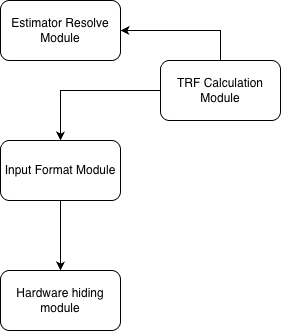
\includegraphics[width=0.5\textwidth]{useHierarchy.png}
\caption{Use hierarchy among modules}
\label{FigUH}
\end{figure}

Figure \ref{FigEstimatorStrategy} provides a more detailed view of the use relations inside the estimator-selection part of the design. The \texttt{TRFExperiment} context depends on the abstract \texttt{Estimator} interface, resolves a concrete strategy from the registry, and then dispatches execution to either the boosting backend or the NCRF backend. This structure keeps estimator-specific policy decisions localized while preserving a single entry point for the overall workflow.

\begin{figure}[H]
\centering
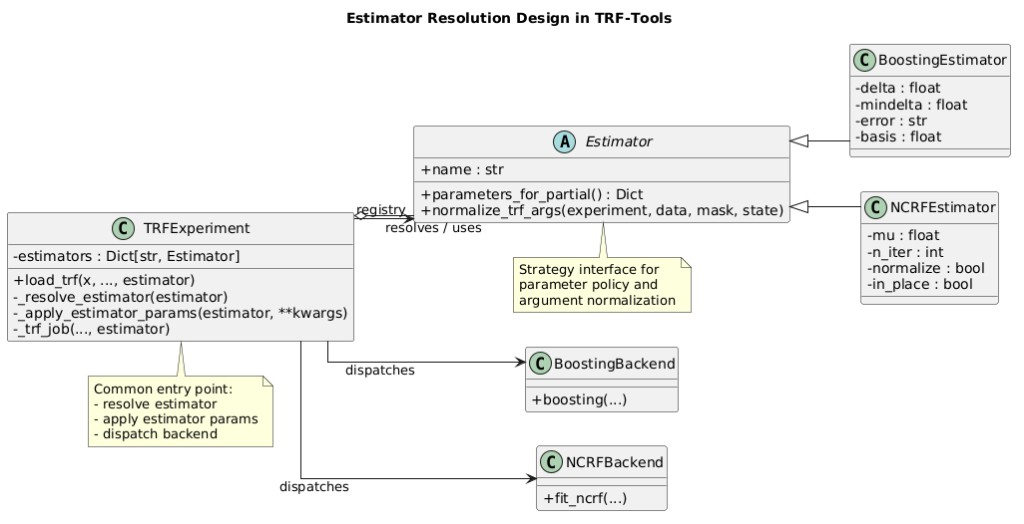
\includegraphics[width=\textwidth]{estimator_strategy_design.png}
\caption{Estimator resolution strategy design in the TRF tools workflow}
\label{FigEstimatorStrategy}
\end{figure}

%\section*{References}

\section{User Interfaces}
NA. The deliverable targets a backend analysis pipeline invoked programmatically
or via scripts; no dedicated GUI or interactive UI is part of the system scope.
% \wss{Design of user interface for software and hardware.  Attach an appendix if
% needed. Drawings, Sketches, Figma}

\section{Design of Communication Protocols}
NA. The system is a single-process analysis pipeline; modules communicate via
in-process function calls and shared data structures, so no external or network
protocol is required.
% \wss{If there is communication between hardware and software, it may be necessary 
% to explain the design of the communication protocol.  This section should be filled 
% in with NA if it is not appropriate for a given project.}

\section{Database Design}
NA
% \wss{If a database is a significant component of the project, the database
% design should be summarized here.  This section should be filled in with NA if
% it is not appropriate for a given project.}

\section{Timeline}
This section lists the timeline of the project.

\begin{table}[H]
  \centering
  \caption{Module Development Timeline}
  \begin{tabular}{l l l l}
  \toprule
  \textbf{Module} & \textbf{ID} & \textbf{Start Date} & \textbf{End Date} \\
  \midrule
  Data Loading Module & \mref{mHH} & 2026-03-16 & 2026-03-19 \\
  Data Preprocessing Module & \mref{mInput} & 2026-03-18 & 2026-03-22 \\
  Estimator Resolution Module & \mref{mEstimator} & 2026-03-21 & 2026-03-26 \\
  TRF Computation Module & \mref{mTRF} & 2026-03-24 & 2026-03-30 \\
  Integration, Testing, and Refinement & -- & 2026-03-28 & 2026-04-02 \\
  \bottomrule
  \end{tabular}
  \end{table}
% \wss{Schedule of tasks and who is responsible}

% \wss{You can point to GitHub if this information is included there}

\bibliographystyle {plainnat}
\bibliography{../../../refs/References}

\newpage{}

\end{document}
